% !TeX program = lualatex
% !TeX encoding = utf8
% !TeX spellcheck = uk_UA
%
% Лекція 1 «Плазма: від іонізованого газу до колективного середовища»
% За розд. 1 книги PlasmaBook (PlasmaBook/Basics/Basics.tex). Рисунки tikz/ — копії з розділу.

\documentclass[]{beamer}
\usetheme{PlasmaPhysics}
\usepackage{PlasmaPhysics}
\setlength{\abovedisplayskip}{3pt}
\setlength{\belowdisplayskip}{3pt}
\setbeamercovered{transparent=25}
\graphicspath{{pictures/}}

\title[Лекції з фізики плазми]{\bfseries\huge Плазма: від іонізованого газу\\ до колективного середовища}
\subtitle{\bfseries Лекції з фізики плазми. Лекція 1}
\author{Пономаренко С. М.}
\date{}

% --- допоміжні команди ---
\newcommand{\fig}[2][\linewidth]{\resizebox{#1}{!}{\input{tikz/#2}}}
\newcommand{\figp}[1]{{\footnotesize\input{tikz/#1}}}
\newcommand{\figw}[1]{\resizebox{\linewidth}{!}{\begin{minipage}{11cm}\centering\input{tikz/#1}\end{minipage}}}
\newcounter{probcnt}
\setcounter{probcnt}{0}
\newcommand{\cm}{\mathrm{см}}
\newcommand{\vT}{v_{T\!e}}

\begin{document}

\usebackgroundtemplate{
	\tikz\node[opacity=0.1]{\includegraphics[width=\paperwidth,height=\paperheight]{background}};%
}

\begin{frame}
	\titlepage
\end{frame}

%% ============================================================
\begin{frame}{План лекції}
	\begin{enumerate}\justifying
		\item Що таке плазма. Види плазми.
		\item Іонізація: формула Саха.
		\item Дві температури.
		\item Квазінейтральність і плазмові коливання.
		\item Дебаївське екранування. Дебаївська сфера.
		\item Слабко- і сильнозв'язана плазма. Три умови плазми.
		\item Екранування у виродженому газі.
		\item Шар біля стінки і зонд Ленгмюра.
	\end{enumerate}
\end{frame}

%% ============================================================
\section{Що таке плазма}
%% ============================================================

\begin{frame}{Що таке плазма?}
	\begin{block}{}\justifying
		\alert{Плазма} --- частково або повністю іонізований газ, у~якому густини
		позитивних і~негативних зарядів практично однакові (\alert{квазінейтральність}),
		а~заряджені частинки поводяться \alert{колективно}.
	\end{block}
	\begin{block}{}\justifying\small
		Термін запропонував І.~Ленгмюр наприкінці 1920-х років (грец. \emph{plasma} --- виліплене,
		оформлене); 1929~р. Л.~Тонкс і~Ленгмюр описали власні коливання електронного газу.
	\end{block}
	\begin{block}{Ступінь іонізації}
		\begin{equation*}
			\alpha=\frac{n_i}{n_i+n_n}
		\end{equation*}
		\small\justifying
		слабо іонізована (частки \%), помірно (кілька \%), повністю ($\alpha\to1$).
	\end{block}
\end{frame}

\begin{frame}{Чим плазма відрізняється від нейтрального газу?}
	\begin{columns}[T]
		\begin{column}{0.48\linewidth}
			\begin{block}{Нейтральний газ}\justifying\small
				Частинки майже вільні, обмінюються імпульсом у~короткочасних парних зіткненнях.
			\end{block}
		\end{column}
		\begin{column}{0.48\linewidth}
			\begin{block}{Плазма}\justifying\small
				Кулонівська сила спадає повільно ($\propto r^{-2}$), а~число частинок у~шарі зростає як $r^2$:
				кожна частинка \alert{одночасно} взаємодіє з~багатьма.
			\end{block}
		\end{column}
	\end{columns}
	\begin{block}{}\justifying\small
		Сила на частинку формується \alert{усередненим полем багатьох частинок}, а~не парними зіткненнями. Звідси
		екранування, плазмові коливання, хвилі й~нестійкості.
	\end{block}
	\begin{block}{}\justifying\small
		Друга особливість --- зв'язок механіки з~електродинамікою: плазма не лише рухається в~полі, а~й~сама
		створює поля та струми, що діють назад на її рух.
	\end{block}
\end{frame}

\begin{frame}{Температура в енергетичних одиницях}
	\begin{block}{}\justifying\small
		$k_{\mathrm B}=1$: температуру пишемо як $T$ і~вимірюємо в~еВ, $1~\text{еВ}\approx11\,600$~К.
		$T$ --- параметр максвеллівського розподілу
		\begin{equation*}
			f\propto\exp\left(-\frac{mv^2}{2T}\right),\qquad
			\left\langle\frac{mv^2}{2}\right\rangle=\frac32\,T.
		\end{equation*}
	\end{block}
	\begin{block}{Числа для оцінок (СГС)}\small
		\begin{equation*}
			e=4{,}8\cdot10^{-10}~\text{СГС},\quad
			e^2\approx1{,}44\cdot10^{-7}~\text{еВ}\cdot\cm,\quad
			1~\text{СГС}=300~\text{В/см}.
		\end{equation*}
	\end{block}
	\begin{exampleblock}{Задача}\small
		Температура поверхні Сонця $5800$~К~$\approx0{,}5$~еВ~$\approx8\cdot10^{-13}$~ерг~$\approx8\cdot10^{-20}$~Дж.
	\end{exampleblock}
\end{frame}

\begin{frame}{Як виникає плазма і які бувають її види}
	\begin{block}{Способи іонізації}\justifying\small
		нагрівання, електричний розряд, фотоіонізація, ударна іонізація, бомбардування частинками.
	\end{block}
	\begin{columns}[T]
		\begin{column}{0.48\linewidth}
			\begin{block}{Низькотемпературна}\small
				$T\lesssim10^5$~К ($\lesssim10$~еВ): розряди, іоносфера, технологічна плазма.
			\end{block}
		\end{column}
		\begin{column}{0.48\linewidth}
			\begin{block}{Високотемпературна}\small
				$T\gtrsim10^6$~К ($\gtrsim100$~еВ); токамаки --- до $10^8$~К~$\approx10$~кеВ. Потрібна для
				\alert{керованого термоядерного синтезу}.
			\end{block}
		\end{column}
	\end{columns}
	\begin{alertblock}{}\justifying\small
		Не плутати з~назвами <<холодна>> і~<<гаряча>> плазма в~теорії хвиль: там ідеться про те, чи істотний
		тепловий рух для даного процесу, а~не про саме значення $T$.
	\end{alertblock}
\end{frame}

\begin{frame}{Діапазон плазм: 25 порядків за концентрацією}
	\begin{table}\centering\scriptsize
		\setlength{\tabcolsep}{3pt}
		\begin{tabular}{lcccc}
			\hline
			Плазма & $n_e$, $\cm^{-3}$ & $T$, еВ & $\lambda_{De}$, см & $N_D$ \\
			\hline
			Іоносфера & $10^{5}$ & $0{,}1$ & $0{,}74$ & $1{,}7\cdot10^{5}$ \\
			Міжзоряний газ & $10$ & $1$ & $2{,}4\cdot10^{2}$ & $5\cdot10^{8}$ \\
			Сонячна корона & $10^{8}$ & $10^{2}$ & $0{,}74$ & $1{,}7\cdot10^{8}$ \\
			Сонячний вітер & $10$ & $10$ & $7{,}4\cdot10^{2}$ & $1{,}7\cdot10^{10}$ \\
			Газовий розряд & $10^{12}$ & $3$ & $1{,}3\cdot10^{-3}$ & $9\cdot10^{3}$ \\
			Токамак & $10^{14}$ & $10^{4}$ & $7{,}4\cdot10^{-3}$ & $1{,}7\cdot10^{8}$ \\
			Ядро Сонця & $10^{26}$ & $10^{3}$ & $2{,}4\cdot10^{-9}$ & $5$ \\
			Електрони в металі & $10^{23}$ & вироджені & --- & --- \\
			\hline
		\end{tabular}
	\end{table}
	\begin{block}{}\justifying\small
		$N_D$ --- число частинок у~дебаївській сфері (див. далі). Ядро Сонця ($N_D\sim5$) --- межа колективного опису;
		електрони в~металі \alert{вироджені} ($T\ll E_F$) і~потребують квантового опису.
	\end{block}
\end{frame}

\begin{frame}{Діаграма $\lg n$--$\lg T$}
	\centering
	\figp{plasma_types.tikz}
	\begin{block}{}\justifying\tiny
		Точка --- плазма з~даними $n$ і~$T$; лінії відокремлюють області, де змінюється фізика: $N_D\sim1$ (межа слабкозв'язаної),
		$T=E_F$ (виродження), $T=m_ec^2$ (релятивізм). Класична ідеальна плазма: $\max\{e^2n^{1/3},\hbar^2n^{2/3}/m_e\}\ll T\ll m_ec^2$.
	\end{block}
\end{frame}

%% ============================================================
\section{Іонізація: формула Саха}
%% ============================================================

\begin{frame}{Скільки енергії потрібно, щоб газ став плазмою?}
	\begin{block}{}\justifying\small
		Іонізація водню $I=13{,}6$~еВ ($1{,}6\cdot10^5$~К), проте газ іонізується помітно за значно нижчих $T$.
		Хімічна рівновага \ce{H <=> p + e} (\,$\mu_a=\mu_i+\mu_e$\,) дає \alert{формулу Саха}:
	\end{block}
	\begin{equation*}
		\tcbhighmath{\frac{n_en_i}{n_n}=\left(\frac{mT}{2\pi\hbar^2}\right)^{3/2}e^{-I/T}\approx2{,}4\cdot10^{15}\,T^{3/2}e^{-I/T}~\cm^{-3}}
	\end{equation*}
	\begin{block}{}\justifying\scriptsize
		У~числовій формі $T$ і~$I$ --- у~кельвінах ($I/k_{\mathrm B}\approx1{,}58\cdot10^5$~К).
		$n_q=(mT/2\pi\hbar^2)^{3/2}=\lambda_{Te}^{-3}$ --- число квантових станів електрона в~одиниці об'єму
		($\lambda_{Te}$ --- теплова довжина хвилі де Бройля).
	\end{block}
\end{frame}

\begin{frame}{Зміст формули Саха}
	\begin{block}{Два множники}\justifying\small
		\begin{enumerate}
			\item $e^{-I/T}$: іонізація помітна вже при $T$ лише в~$10$--$20$ разів меншій за $I$.
			\item $n_q\gg n$: на кожен електрон припадає величезна кількість вільних станів ($n_q/n\sim10^6$--$10^{10}$),
			виграш \alert{ентропії} перекриває больцманівський множник.
		\end{enumerate}
	\end{block}
	\begin{alertblock}{Наслідок}\justifying\small
		За однакової температури \emph{чим розрідженіший газ, тим легше він іонізується}.
	\end{alertblock}
	\begin{exampleblock}{Оцінка: кімнатна температура}\justifying\small
		$T=0{,}026$~еВ, $I=14{,}6$~еВ, $n\approx3\cdot10^{19}~\cm^{-3}$: $e^{-I/T}\sim10^{-244}$, $\alpha\sim10^{-122}$.
		А~водень при $1$~еВ і~$10^{17}~\cm^{-3}$ іонізований уже на~$\sim20\,\%$.
	\end{exampleblock}
\end{frame}

\begin{frame}{Ступінь іонізації водню}
	\begin{columns}[T]
		\begin{column}{0.46\linewidth}
			\begin{block}{}\justifying\scriptsize
				$n_e=n_i=\alpha n$, $n_n=(1-\alpha)n$:
				\begin{equation*}
					\frac{\alpha^2}{1-\alpha}=\frac{n_q}{n}\,e^{-I/T}.
				\end{equation*}
				Для $n=10^{17}~\cm^{-3}$:
				\begin{equation*}
					\begin{aligned}
						\alpha&\approx1{,}3\cdot10^{-4}&&(0{,}5~\text{еВ}),\\
						\alpha&\approx0{,}18&&(1~\text{еВ}),\\
						\alpha&\approx0{,}99&&(2~\text{еВ}).
					\end{aligned}
				\end{equation*}
			\end{block}
			\begin{alertblock}{}\justifying\scriptsize
				Перехід \alert{плавний} (кросовер), не фазовий. У~розрядах і~під випромінюванням $\alpha$ може бути
				нерівноважним.
			\end{alertblock}
		\end{column}
		\begin{column}{0.52\linewidth}
			\figw{saha-curve.tikz}
		\end{column}
	\end{columns}
\end{frame}

%% ============================================================
\section{Дві температури}
%% ============================================================

\begin{frame}{Температура плазми та два компоненти}
	\begin{block}{}\justifying\small
		Електрони й~іони можуть мати різні температури $T_e$ і~$T_i$ (\alert{двотемпературна плазма}).
	\end{block}
	\begin{block}{Чому часто $T_e>T_i$}\justifying\small
		Енергію від поля отримують електрони. При пружному зіткненні з~іоном електрон віддає лише
		\begin{equation*}
			\frac{\delta E}{E}\le\frac{4m_em_i}{(m_e+m_i)^2}\approx\frac{4m_e}{m_i}\approx0{,}2\,\%
		\end{equation*}
		(як тенісний м'ячик від вантажівки).
	\end{block}
	\begin{exampleblock}{Приклад}\justifying\small
		Позитивний стовп тліючого розряду ($\sim0{,}1$~мм рт.~ст.): $T_e\sim1$--$3$~еВ, а~іони --- кілька сотень кельвінів.
		Спершу встановлюється максвелівський розподіл електронів, потім іонів, і~лише згодом --- рівність $T_e=T_i$.
	\end{exampleblock}
\end{frame}

%% ============================================================
\section{Квазінейтральність і плазмові коливання}
%% ============================================================

\begin{frame}{Квазінейтральність}
	\begin{block}{}\justifying\small
		Розділення зарядів дає поле (теорема Гаусса)
		\begin{equation*}
			\nabla\cdot\vec E=4\pi e\,(Zn_i-n_e).
		\end{equation*}
		Питомий заряд електрона $e/m_e$ величезний, тому електрони швидко компенсують розділення:
		\begin{equation*}
			\tcbhighmath{\rho=e(Zn_i-n_e)\approx0\quad\Rightarrow\quad n_e\approx Zn_i}
		\end{equation*}
	\end{block}
	\begin{exampleblock}{Оцінка}\justifying\scriptsize
		$n=10^{12}~\cm^{-3}$, $L=1$~см, розділення лише $1\,\%$: $E\sim4\pi e\,\delta n\,L\approx2\cdot10^4$~В/см,
		тоді як тепловому руху ($T=1$~еВ) відповідає $T/eL\sim1$~В/см. Навіть $\delta n/n\sim10^{-6}$ дає
		$E\sim2$~В/см --- порівнянне з~тепловим.
	\end{exampleblock}
	\begin{alertblock}{}\justifying\scriptsize
		Це макроскопічне наближення, а~не нуль у~кожній точці: локальні відхилення лежать в~основі
		екранування й~плазмових коливань.
	\end{alertblock}
\end{frame}

\begin{frame}{Плазмові коливання: модель}
	\begin{columns}[T]
		\begin{column}{0.5\linewidth}
			\begin{block}{}\justifying\scriptsize
				Електрони плоского шару зміщені як ціле на $x$ відносно нерухомого іонного фону. На краях ---
				поверхневі заряди $\sigma=\mp n_eex$, між ними поле конденсатора
				\begin{equation*}
					E=4\pi n_eex.
				\end{equation*}
			\end{block}
			\begin{block}{}\scriptsize
				\begin{equation*}
					m_e\ddot x=-eE=-4\pi n_ee^2x
				\end{equation*}
			\end{block}
		\end{column}
		\begin{column}{0.48\linewidth}
			\centering
			\resizebox{!}{3.2cm}{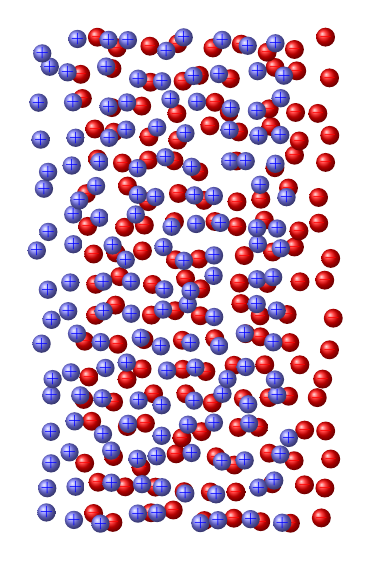
\begin{tikzpicture}[scale=0.75,
		ions/.style={
				circle, ball color=blue!50, font=\tiny, inner sep=0, blue
			},
		electrons/.style={
				circle, ball color=red, font=\tiny, inner sep=0, red
			},
	]

	%        \draw[xshift=0.5cm, fill=gray!50] (0,0) rectangle ++(4,8);
	%        \draw[dashed] (0,0) rectangle ++(4,8);

	\foreach \x in {0,0.5,...,4} {
			\foreach \y in {0,0.5,...,8} {
					\node[ions] at (\x+0.3*rnd,\y+0.3*rnd) {$+$};
					\node[electrons] at ({\x+0.75+0.3*rnd},\y+0.3*rnd) {$-$};
				}
		}
\end{tikzpicture}}\\[0.3em]
			\resizebox{!}{2.6cm}{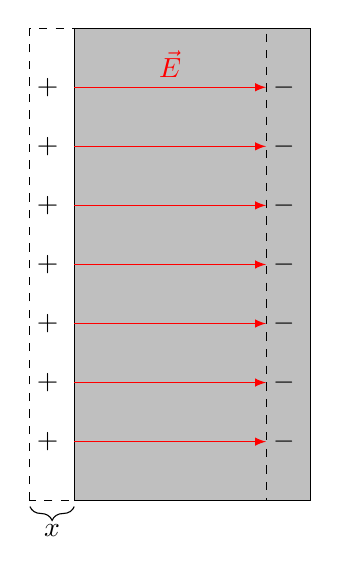
\begin{tikzpicture}[scale=0.75,
		ions/.style={
				circle, ball color=blue!50, font=\tiny, inner sep=0, blue
			},
		electrons/.style={
				circle, ball color=red, font=\tiny, inner sep=0, red
			},
	]

	\draw[xshift=0.75cm, fill=gray!50] (0,0) rectangle ++(4,8);
	\draw[dashed] (0,0) rectangle ++(4,8);

	\foreach \y in {1,...,7} {
			\node at (0.3, \y) {$+$};
			\node at (4.3, \y) {$-$};
			\draw[-latex, red] (0.75, \y) -- (4, \y) \ifnum\y=7 node[above, pos=0.5] {$\vec{E}$} \fi ;
		}

	\draw[decorate,decoration={brace,amplitude=5pt,mirror,raise=0ex}] (0,-0.1)  -- (0.75,-0.1)
	node[midway, yshift=-2ex] {$x$};

\end{tikzpicture}}
		\end{column}
	\end{columns}
\end{frame}

\begin{frame}{Плазмова частота}
	\begin{equation*}
		\ddot x+\omega_{pe}^2x=0,\qquad
		\tcbhighmath{\omega_{pe}=\sqrt{\frac{4\pi n_ee^2}{m_e}}\approx5{,}64\cdot10^4\sqrt{n_e[\cm^{-3}]}~\text{с}^{-1}}
	\end{equation*}
	\begin{block}{Без уявного конденсатора}\justifying\small
		З~рівняння неперервності, $m_e\partial_t\vec v=-e\vec E$ і~$\nabla\cdot\vec E=4\pi\rho$:
		\begin{equation*}
			\frac{\partial^2\rho}{\partial t^2}+\omega_{pe}^2\rho=0.
		\end{equation*}
		Порушення нейтральності саме коливається з~частотою $\omega_{pe}$.
	\end{block}
	\begin{block}{}\justifying\small
		$\omega_{pe}$ --- частота, з~якою плазма відновлює квазінейтральність; $\omega_{pe}^{-1}$ --- час відновлення
		($n=10^{12}~\cm^{-3}$: $\sim2\cdot10^{-11}$~с). Іонний внесок: $\omega_{pi}^2/\omega_{pe}^2=m_e/m_i$, тож $\omega_p\equiv\omega_{pe}$.
	\end{block}
\end{frame}

\begin{frame}{Два масштаби колективної реакції}
	\begin{block}{}\justifying\small
		За час $\omega_{pe}^{-1}$ тепловий електрон проходить відстань
		\begin{equation*}
			\tcbhighmath{\lambda_{De}=\frac{\vT}{\omega_{pe}},\qquad
			\vT=\sqrt{\frac{T_e}{m_e}}\approx4{,}2\cdot10^7\sqrt{T_e[\text{еВ}]}~\text{см/с}}
		\end{equation*}
	\end{block}
	\begin{block}{}\justifying\small
		На масштабах $<\lambda_{De}$ плазма <<не встигає>> колективно відповісти: електрон вилітає з~області раніше,
		ніж поле його поверне. Отже, колективну реакцію задають
		\begin{itemize}
			\item час $\sim\omega_{pe}^{-1}$,
			\item довжина $\sim\lambda_{De}$.
		\end{itemize}
	\end{block}
	\begin{exampleblock}{Задача}\small
		Час відновлення $\lambda_{De}/\vT$: іоносфера $\approx6\cdot10^{-8}$~с, токамак $\approx2\cdot10^{-12}$~с.
	\end{exampleblock}
\end{frame}

%% ============================================================
\section{Дебаївське екранування}
%% ============================================================

\begin{frame}{Дебаївське екранування: постановка}
	\begin{columns}[T]
		\begin{column}{0.58\linewidth}
			\begin{block}{}\justifying\small
				Внесемо пробний заряд $q$. У~вакуумі його поле спадає як $1/r$ і~сягає далеко. У~плазмі рухливі
				частинки протилежного знака притягуються, однойменного --- відштовхуються.
			\end{block}
			\begin{block}{}\justifying\small
				Заряд оточується <<шубою>>, поле послаблюється. Тепловий рух не дає шубі стиснутися в~точку:
				вона розмазана на $\sim\lambda_D$, а~її повний заряд дорівнює $-q$.
			\end{block}
		\end{column}
		\begin{column}{0.4\linewidth}
			\fig{debye_sphere.tikz}
		\end{column}
	\end{columns}
\end{frame}

\begin{frame}{Дебаївське екранування: вивід}
	\begin{overprint}
		\onslide<1>
		\begin{block}{1. Розподіл Больцмана}\justifying\small
			Для кожного сорту $s$ у~потенціалі $\varphi(\vec r)$:
			\begin{equation*}
				n_s=n_{s0}\exp\left(-\frac{q_s\varphi}{T_s}\right),\qquad\sum_sq_sn_{s0}=0.
			\end{equation*}
			Густина заряду $\rho=\sum_sq_sn_{s0}\exp(-q_s\varphi/T_s)$.
		\end{block}
		\onslide<2>
		\begin{block}{2. Слабке поле $|q_s\varphi|\ll T_s$}\justifying\small
			Нульовий доданок зникає завдяки нейтральності:
			\begin{equation*}
				\rho\simeq-\varphi\sum_s\frac{n_{s0}q_s^2}{T_s}.
			\end{equation*}
		\end{block}
		\onslide<3>
		\begin{block}{3. Рівняння Пуассона з пробним зарядом}\justifying\small
			\begin{equation*}
				\Delta\varphi-\frac{\varphi}{\lambda_D^2}=-4\pi q\,\delta(\vec r),\qquad
				\tcbhighmath{\frac{1}{\lambda_D^2}=4\pi\sum_s\frac{n_{s0}q_s^2}{T_s}}
			\end{equation*}
			$\lambda_D$ --- \alert{дебаївська довжина} (радіус екранування).
		\end{block}
		\onslide<4>
		\begin{block}{4. Сферична симетрія}\justifying\small
			При $r>0$: $\Delta\varphi=\frac1r\frac{d^2(r\varphi)}{dr^2}$, $u=r\varphi$:
			\begin{equation*}
				u''=\frac{u}{\lambda_D^2}\ \Rightarrow\ u=Ae^{-r/\lambda_D}+Be^{r/\lambda_D}.
			\end{equation*}
			$\varphi\to0$ при $r\to\infty$ дає $B=0$; поблизу заряду $\varphi\to q/r$ дає $A=q$.
		\end{block}
	\end{overprint}
\end{frame}

\begin{frame}{Екранований потенціал}
	\begin{columns}[T]
		\begin{column}{0.5\linewidth}
			\begin{equation*}
				\tcbhighmath{\varphi(r)=\frac qr\,e^{-r/\lambda_D}}
			\end{equation*}
			\begin{block}{}\justifying\scriptsize
				Кулонівське поле експоненціально послаблюється на $\sim\lambda_D$ (Дебай і~Хюккель, 1923~р.,
				електроліти; плазма --- найчистіший прояв).
			\end{block}
			\begin{block}{Заряд <<шуби>>}\justifying\scriptsize
				\begin{equation*}
					\int\rho\,4\pi r^2dr=-\frac q{\lambda_D^2}\int_0^\infty re^{-r/\lambda_D}dr=-q
				\end{equation*}
				Для спостерігача на $r\gg\lambda_D$ заряд з~оболонкою практично нейтральний.
			\end{block}
		\end{column}
		\begin{column}{0.48\linewidth}
			\centering% Версія рис. потенціалу для слайда: r у одиницях lambda_D, підписи без налізання.
\begin{tikzpicture}
	\begin{axis}[
		width=6.2cm, height=5.6cm,
		axis lines=middle, clip=false,
		xmin=0, xmax=3.6, ymin=0, ymax=5,
		xtick={1,2,3}, xticklabels={$\lambda_D$,$2\lambda_D$,$3\lambda_D$},
		ytick=\empty,
		xlabel={$r$}, ylabel={$\varphi$},
		every axis x label/.style={at={(current axis.right of origin)},anchor=west},
		every axis y label/.style={at={(current axis.north west)},above=1mm},
		]
		\addplot[red!70!black, dashed, thick, domain=0.2:3.4, samples=100] {1/x};
		\addplot[blue!70!black, thick, domain=0.2:3.4, samples=200] {exp(-x)/x};
		\node[red!70!black, anchor=west] at (axis cs:0.75,4.3) {$\dfrac qr$ (вакуум)};
		\node[blue!70!black, anchor=west] at (axis cs:1.25,2.0) {$\dfrac qr\,e^{-r/\lambda_D}$};
		\fill[red, opacity=0.4] (axis cs:0,0) circle (3pt);
	\end{axis}
\end{tikzpicture}

		\end{column}
	\end{columns}
\end{frame}

\begin{frame}{Скільки сортів частинок екранує?}
	\begin{block}{}\small
		Електрони й~однозарядні іони:
		\begin{equation*}
			\frac1{\lambda_D^2}=\frac1{\lambda_{De}^2}+\frac1{\lambda_{Di}^2},\qquad
			\lambda_{De,i}=\sqrt{\frac{T_{e,i}}{4\pi n_{e,i}e^2}}
		\end{equation*}
		\justifying
		При $T_e=T_i$: $\lambda_D=\lambda_{De}/\sqrt2$. Практично $\lambda_{De}\approx743\sqrt{T_e[\text{еВ}]/n_e[\cm^{-3}]}$~см.
	\end{block}
	\begin{alertblock}{}\justifying\small
		Обидва сорти мають встигнути перебудуватися: процес повільний порівняно з~$\lambda_D/v_{Ti}$.
		Для швидкого процесу іони нерухомі, екранують лише електрони --- береться $\lambda_{De}$.
		При $T_i\ll T_e$ для повільного процесу $\lambda_D\approx\lambda_{Di}\ll\lambda_{De}$.
	\end{alertblock}
	\begin{exampleblock}{Задача}\small
		$n=10^{12}~\cm^{-3}$, $T_e=3$~еВ, $T_i=0{,}03$~еВ: $\lambda_{De}\approx1{,}3\cdot10^{-3}$~см,
		$\lambda_{Di}\approx1{,}3\cdot10^{-4}$~см, $\lambda_D\approx\lambda_{Di}$.
	\end{exampleblock}
\end{frame}

\begin{frame}{Умови застосовності. Квазінейтральність і розмір системи}
	\begin{block}{Лінеаризація}\justifying\small
		Потрібно $|q\varphi|\ll T$ при $r\gtrsim\lambda_D$. Для $q=e$ це $e^2/\lambda_D\ll T$, тобто з~точністю до множника
		\begin{equation*}
			\frac1{N_D}\ll1:
		\end{equation*}
		у~сфері радіуса $\lambda_D$ має бути \alert{багато частинок}.
	\end{block}
	\begin{block}{Розмір системи $L$}\justifying\small
		Неоднорідність $\delta n$ на масштабі $L$: $\varphi/L^2\sim4\pi e\,\delta n$, $\varphi\lesssim T/e$, звідки
		\begin{equation*}
			\frac{\delta n}n\lesssim\left(\frac{\lambda_{De}}L\right)^2,\qquad
			\tcbhighmath{\lambda_D\ll L}
		\end{equation*}
		Біля стінок і~електродів ця умова порушується --- там \alert{дебаївські шари}.
	\end{block}
\end{frame}

%% ============================================================
\section{Дебаївська сфера. Колективність}
%% ============================================================

\begin{frame}{Дебаївська сфера і умова колективності}
	\begin{block}{}\justifying\small
		\alert{Дебаївська сфера} --- область радіуса $\lambda_{De}$ навколо частинки. Число електронів у~ній:
		\begin{equation*}
			\tcbhighmath{N_D=\frac{4\pi}{3}\,n_e\lambda_{De}^3}
		\end{equation*}
	\end{block}
	\begin{block}{Умова колективності}\justifying\small
		\begin{equation*}
			N_D\gg1\quad\Longleftrightarrow\quad\lambda_D\gg a,\qquad a\sim n^{-1/3}.
		\end{equation*}
		Поле визначається сумарною дією багатьох частинок, а~не одним сусідом: екранування колективне.
	\end{block}
	\begin{block}{Спостережуваний наслідок}\justifying\small
		Частота парних зіткнень $\nu\sim\omega_p\ln N_D/N_D\ll\omega_p$: колективні ефекти домінують над парними.
	\end{block}
\end{frame}

\begin{frame}{Інтуїція часто працює навпаки}
	\begin{alertblock}{Хибна думка}\justifying\small
		<<Багато частинок у~сфері --- вони сильно взаємодіють і~постійно б'ються; мало --- частинки вільні>>.
	\end{alertblock}
	\begin{exampleblock}{Насправді}\justifying\small
		\emph{Багато частинок у~сфері $\Rightarrow$ кожен сусід діє слабко.} Сфера велика, бо плазма гаряча
		і~(або) розріджена ($\lambda_{De}^2=T/4\pi ne^2$): сусіди далеко, потенціальна енергія $e^2/a\ll T$.
		Сила на частинку --- сума сотень крихітних внесків, що згладжуються в~спільне поле.
	\end{exampleblock}
	\begin{block}{}\justifying\small
		\emph{Мало частинок ($N_D\lesssim1$) $\Rightarrow$ сусід діє сильно:} хмари немає, поле сусіда на $a$ голе кулонівське,
		$e^2/a\gtrsim T$. Ідеальна плазма --- газ майже вільних частинок у~гладкому полі всіх інших; кореляції дають
		поправки $\sim1/N_D$.
	\end{block}
\end{frame}

\begin{frame}{Перекриття дебаївських сфер}
	\centering
	\resizebox{!}{4.2cm}{% Рис.: одна й та сама дебаївська сфера, але різне число частинок у ній.
% (а) N_D >> 1: поле = сума багатьох слабких внесків; (б) N_D ~ 1: переважає пара з найближчим сусідом.
\begin{tikzpicture}[
		ion/.style={circle, fill=blue!60, inner sep=0pt, minimum size=4pt},
		el/.style={circle, fill=red!70, inner sep=0pt, minimum size=4pt},
		test/.style={circle, ball color=blue!50, inner sep=2.2pt, font=\scriptsize, text=white},
		lab/.style={font=\footnotesize, anchor=north},
	]
	\def\R{1.7}
	\pgfmathsetseed{7}
	%% ---------- (а) густо: N_D >> 1 ----------
	\begin{scope}
		\path[inner color=red!25, outer color=white] (0,0) circle(\R+0.3);
		\draw[thick, dashed, gray!70!black] (0,0) circle(\R);
		\def\sp{0.36}
		\foreach \ix in {-5,...,5}{
			\foreach \iy in {-5,...,5}{
				\pgfmathsetmacro{\px}{\ix*\sp+(rnd-0.5)*0.7*\sp}
				\pgfmathsetmacro{\py}{\iy*\sp+(rnd-0.5)*0.7*\sp}
				\pgfmathsetmacro{\rr}{veclen(\px,\py)}
				\ifdim\rr pt<\R pt
					\ifdim\rr pt>0.2pt
						\pgfmathtruncatemacro{\sgn}{mod(\ix+\iy+10,2)}
						\ifnum\sgn=0
							\draw[gray!45, line width=0.2pt] (0,0)--(\px,\py);
							\node[el] at (\px,\py) {};
						\else
							\draw[gray!45, line width=0.2pt] (0,0)--(\px,\py);
							\node[ion] at (\px,\py) {};
						\fi
					\fi
				\fi
			}
		}
		\node[test] at (0,0) {$+$};
		\draw[<->, thick] (0,0)--(35:\R) node[midway, above, sloped, font=\footnotesize] {$\lambda_D$};
		% відстань a надто мала для стрілки в масштабі рисунка: показуємо збільшений фрагмент
		\draw[gray!70!black, thin] (-3.3,0.2) circle(0.62);
		\node[ion, minimum size=5pt] at (-3.3-0.3,0.2) {};
		\node[el, minimum size=5pt] at (-3.3+0.3,0.2) {};
		\draw[<->, thick] (-3.3-0.3,-0.05)--(-3.3+0.3,-0.05) node[midway, below, font=\footnotesize] {$a$};
		\node[font=\scriptsize, gray!50!black, align=center] at (-3.3,1.2) {збільшений\\ фрагмент};
		\node[lab] at (0,-\R-1.0) {\textbf{(а)} $\lambda_D\gg a$};
	\end{scope}
	%% ---------- (б) рідко: N_D ~ 1 ----------
	\begin{scope}[xshift=6.0cm]
		\draw[thick, dashed, gray!70!black] (0,0) circle(\R);
		\def\sp{1.45}
		\foreach \ix in {-2,...,2}{
			\foreach \iy in {-2,...,2}{
				\pgfmathsetmacro{\px}{\ix*\sp+(rnd-0.5)*0.5*\sp}
				\pgfmathsetmacro{\py}{\iy*\sp+(rnd-0.5)*0.5*\sp}
				\pgfmathsetmacro{\rr}{veclen(\px,\py)}
				\ifdim\rr pt<\R pt
					\ifdim\rr pt>0.2pt
						\pgfmathtruncatemacro{\sgn}{mod(\ix+\iy+10,2)}
						\ifnum\sgn=0
							\draw[black!70, line width=0.9pt] (0,0)--(\px,\py);
							\node[el] at (\px,\py) {};
						\else
							\draw[black!70, line width=0.9pt] (0,0)--(\px,\py);
							\node[ion] at (\px,\py) {};
						\fi
					\fi
				\fi
			}
		}
		\node[test] at (0,0) {$+$};
		\draw[<->, thick] (0,0)--(35:\R) node[midway, above, sloped, font=\footnotesize] {$\lambda_D$};
		\draw[<->, thick] (-\R+0.0,-\R-0.45)--(-\R+\sp,-\R-0.45) node[midway, below, font=\footnotesize] {$a$};
		\node[lab] at (0,-\R-1.0) {\textbf{(б)} $\lambda_D\sim a$};
	\end{scope}
\end{tikzpicture}
}
	\begin{columns}[T]
		\begin{column}{0.48\linewidth}
			\begin{block}{}\justifying\tiny
				(а) $\lambda_D\gg a$: сфери сусідів \alert{перекриваються}, кожна точка лежить у~$N_D$ сферах; поле --- гладкий результат багатьох слабких внесків.
				(б) $\lambda_D\lesssim a$: сфери окремі, переважають парні взаємодії --- сильний зв'язок.
			\end{block}
		\end{column}
		\begin{column}{0.48\linewidth}
			\begin{alertblock}{}\justifying\tiny
				Хмара несе заряд $-e$ --- надлишок лише \emph{однієї} частинки серед $N_D$ при флуктуаціях $\sim\sqrt{N_D}$. На миттєвому знімку її не видно: вона існує в~середньому.
			\end{alertblock}
		\end{column}
	\end{columns}
\end{frame}

%% ============================================================
\section{Слабко- і сильнозв'язана плазма}
%% ============================================================

\begin{frame}{Параметр зв'язку}
	\begin{block}{}\justifying\small
		Порівняємо кулонівську енергію сусідів $U_{\mathrm C}\sim e^2/a$ з~тепловою $U_T\sim T$:
		\begin{equation*}
			\tcbhighmath{\Gamma=\frac{U_{\mathrm C}}{U_T}=\frac{e^2}{a\,T},\qquad a=n^{-1/3}}
		\end{equation*}
	\end{block}
	\begin{columns}[T]
		\begin{column}{0.48\linewidth}
			\begin{block}{$\Gamma\ll1$}\justifying\small
				\alert{слабкозв'язана} плазма: $N_D\gg1$, екранування колективне, $p\simeq\sum_sn_sT_s$.
			\end{block}
		\end{column}
		\begin{column}{0.48\linewidth}
			\begin{block}{$\Gamma\gtrsim1$}\justifying\small
				\alert{сильнозв'язана}: рух корельований, дебаївське екранування не працює.
			\end{block}
		\end{column}
	\end{columns}
\end{frame}

\begin{frame}{Зв'язок $N_D$ і $\Gamma$}
	\begin{block}{}\small
		Із $T=e^2n^{1/3}/\Gamma$: $\lambda_{De}^2=1/(4\pi n^{2/3}\Gamma)$, звідки
		\begin{equation*}
			\tcbhighmath{N_D=\frac{1}{6\sqrt\pi}\,\Gamma^{-3/2}\approx0{,}09\,\Gamma^{-3/2}},\qquad
			\frac{\lambda_{De}}{a}=\frac{1}{\sqrt{4\pi\Gamma}}.
		\end{equation*}
	\end{block}
	\begin{block}{Числа: що означає <<$\ll$>>}\justifying\small
		$\Gamma=0{,}01\Rightarrow N_D\approx90$;\quad $\Gamma=0{,}07\Rightarrow N_D\approx5$;\quad $\Gamma=1\Rightarrow N_D\approx0{,}1$.
		Для $N_D\gtrsim100$ потрібно $\Gamma\lesssim0{,}01$.
	\end{block}
	\begin{exampleblock}{Ядро Сонця}\justifying\small
		$\Gamma\approx0{,}07$, $N_D\approx5$: все ще плазма, але колективний опис лише наближений (поправки $\sim1/N_D\sim0{,}2$).
	\end{exampleblock}
\end{frame}

\begin{frame}{Три умови плазми}
	\begin{enumerate}\justifying
		\item[1.] $N_D\gg1$ --- \alert{колективність} екранування (еквівалентно $\Gamma\ll1$).
		\vspace*{0.5em}
		\item[2.] $\lambda_D\ll L$ --- \alert{квазінейтральність} на масштабі системи.
		\vspace*{0.5em}
		\item[3.] $\omega_p\tau\gg1$ --- плазма поводиться як плазма, а~не як нейтральний газ: за $1/\omega_p$ встигає
		колективна відповідь, а~заряджена частинка не зіткнулася з~нейтральним атомом ($\tau$ --- час між зіткненнями
		з~нейтральними).
	\end{enumerate}
	\begin{alertblock}{}\justifying\small
		Слабко іонізований газ із~частими зіткненнями з~нейтральними атомами веде себе як звичайний газ, хоча $N_D\gg1$.
	\end{alertblock}
\end{frame}

%% ============================================================
\section{Екранування у виродженому газі}
%% ============================================================

\begin{frame}{Довжина Томаса--Фермі}
	\begin{block}{}\justifying\small
		Екранування вимагає лише чутливості концентрації до потенціалу, $\delta n=(\partial n/\partial\mu)\,e\varphi$:
		\begin{equation*}
			\frac1{\lambda^2}=4\pi e^2\,\frac{\partial n}{\partial\mu}.
		\end{equation*}
	\end{block}
	\begin{columns}[T]
		\begin{column}{0.48\linewidth}
			\begin{block}{Невироджений: $n\propto e^{\mu/T}$}\small
				$\partial n/\partial\mu=n/T\ \Rightarrow\ \lambda_{De}$.
			\end{block}
		\end{column}
		\begin{column}{0.48\linewidth}
			\begin{block}{Вироджений: $n\propto\mu^{3/2}$}\small
				$\partial n/\partial\mu=3n/2E_F$.
			\end{block}
		\end{column}
	\end{columns}
	\begin{equation*}
		\tcbhighmath{\lambda_{TF}=\sqrt{\frac{E_F}{6\pi ne^2}}\approx0{,}5\sqrt{a_Bn^{-1/3}}},\qquad a_B=0{,}53\cdot10^{-8}~\text{см}
	\end{equation*}
	\begin{exampleblock}{Мідь}\justifying\small
		$n\approx8{,}5\cdot10^{22}~\cm^{-3}$, $E_F\approx7$~еВ: $\lambda_{TF}\approx0{,}55\cdot10^{-8}$~см --- частка міжатомної відстані.
		Саме тому добре працює наближення <<заряд на поверхні провідника>>.
	\end{exampleblock}
\end{frame}

%% ============================================================
\section{Шар біля стінки і зонд Ленгмюра}
%% ============================================================

\begin{frame}{Заряджена поверхня: шар Гуї--Чепмена}
	\begin{columns}[T]
		\begin{column}{0.5\linewidth}
			\begin{block}{}\justifying\scriptsize
				Півпростір $x>0$ --- плазма, площина $x=0$ з~густиною заряду $\sigma>0$. За Больцманом
				$\rho=-2ne\sinh(e\varphi/T)$. Інтеграл енергії (множимо на $2E$) дає
				\begin{equation*}
					\tanh\frac{e\varphi}{4T}=\tanh\frac{e\varphi_0}{4T}\,e^{-x/\lambda_D}
				\end{equation*}
				$e\varphi_0\ll T$: $\varphi=\varphi_0e^{-x/\lambda_D}$, $\varphi_0=4\pi\sigma\lambda_D$.
			\end{block}
			\begin{alertblock}{}\justifying\scriptsize
				$e\varphi_0\gg T$: біля поверхні $\varphi\approx(2T/e)\ln(2\lambda_D/x)$, потенціал <<насичується>>; товщина
				$\sim\lambda_D$ лишається лише при $e\varphi_0\lesssim T$.
			\end{alertblock}
		\end{column}
		\begin{column}{0.48\linewidth}
			\fig{debye-layer.tikz}
		\end{column}
	\end{columns}
\end{frame}

\begin{frame}{Шар біля поглинальної стінки}
	\begin{columns}[T]
		\begin{column}{0.46\linewidth}
			\begin{enumerate}\justifying\scriptsize
				\item Електрони швидші за іони ($v_{Te}/v_{Ti}\sim\sqrt{m_i/m_e}$): стінка заряджається \alert{негативно}.
				\item Вона відштовхує електрони від шару $\sim\lambda_D$: там $n_i>n_e$ --- шар додатного об'ємного заряду.
				\item Поле спрямоване до стінки: відштовхує електрони, прискорює іони.
			\end{enumerate}
			\begin{block}{}\justifying\scriptsize
				Від шару залежать струм на зонд і~потоки частинок та~енергії на будь-яку поверхню (у~реакторі --- нагрів і~розпилення першої стінки).
			\end{block}
		\end{column}
		\begin{column}{0.52\linewidth}
			\fig{sheath.tikz}
		\end{column}
	\end{columns}
\end{frame}

\begin{frame}{Критерій Бома}
	\begin{equation*}
		\tcbhighmath{u_0\ge c_s,\qquad c_s=\sqrt{\frac{T_e}{m_i}}\quad(T_i\ll T_e,\ Z=1)}
	\end{equation*}
	\begin{block}{Чому саме так}\justifying\small
		Шар існує лише при $n_i>n_e$. Електрони: $n_e\propto\exp(e\varphi/T_e)$ --- швидкість спадання фіксована. Іони: $n_iu=\text{const}$, і~що
		повільніше іон входить, то швидше падає $n_i$. При $u_0<c_s$ густина іонів падає швидше за електронну: $n_i<n_e$, шару немає.
	\end{block}
	\begin{block}{Передшар}\justifying\small
		Іони набирають $c_s$ в~квазінейтральному передшарі, падіння потенціалу $\gtrsim T_e/2e$, $n_{\mathrm{sh}}=n_0e^{-1/2}\approx0{,}61\,n_0$.
	\end{block}
	\begin{block}{}\small
		Вивід --- в~задачі до розділу (лінеаризація рівняння Пуассона біля межі шару).
	\end{block}
\end{frame}

\begin{frame}{Плаваючий потенціал і потік енергії на стінку}
	\begin{block}{}\justifying\small
		Струм дорівнює нулю: $\Gamma_i=n_0e^{-1/2}c_s$ і $\Gamma_e=\tfrac14n_0\bar v_e\exp(e\varphi_f/T_e)$, $\bar v_e=\sqrt{8T_e/\pi m_e}$:
		\begin{equation*}
			\tcbhighmath{\varphi_f=-\frac{T_e}{2e}\left(\ln\frac{m_i}{2\pi m_e}+1\right)}
		\end{equation*}
		Водень: $\varphi_f\approx-3{,}3\,T_e/e$; дейтерій: $\approx-3{,}7\,T_e/e$.
	\end{block}
	\begin{block}{Товщина шару і потік енергії}\justifying\small
		Дебаївський шар (закон Чайлда--Ленгмюра, $\varphi\propto x^{4/3}$): товщина $\approx2\lambda_{De}$. Потік енергії
		\begin{equation*}
			Q\approx\gamma T_e\,\Gamma_i,\qquad\gamma\approx2+\frac{e|\varphi_f|}{T_e}+\frac{2{,}5\,T_i}{T_e}\ \ (7\text{--}8\ \text{для водню, }T_i\sim T_e).
		\end{equation*}
	\end{block}
\end{frame}

\begin{frame}{Зонд Ленгмюра: схема і ВАХ}
	\begin{columns}[T]
		\begin{column}{0.5\linewidth}
			\fig{probe-circuit.tikz}
			\begin{block}{}\justifying\scriptsize
				Малий електрод з~напругою $V$ відносно стінки; змінюючи $V$, знімають $I(V)$. У~дроті течуть електрони: електронний струм з~плазми
				--- додатний, іонний --- від'ємний.
			\end{block}
		\end{column}
		\begin{column}{0.48\linewidth}
			\figw{probe-iv.tikz}
		\end{column}
	\end{columns}
\end{frame}

\begin{frame}{Три ділянки ВАХ}
	\begin{table}\centering\scriptsize
		\setlength{\tabcolsep}{3pt}
		\renewcommand{\arraystretch}{1.5}
		\begin{tabular}{p{2.3cm}p{4.2cm}p{2.6cm}}
			\hline
			Ділянка & Що відбувається & Що отримуємо \\
			\hline
			$V\ll V_f$: іонне насичення & лише іони; $I_{is}\approx0{,}6\,e\,n_0c_sS$ & $n_0$ (при відомому $T_e$) \\
			$V_f<V<V_p$: гальмівна & $I_e\propto\exp\bigl(e(V-V_p)/T_e\bigr)$ & $T_e$: $d\ln I_e/dV=e/T_e$ \\
			$V\ge V_p$: електронне насичення & весь тепловий потік: $I_{es}=\tfrac14en_0\bar v_eS$ & $V_p$ (злам); перевірка $n_0$ \\
			\hline
		\end{tabular}
	\end{table}
	\begin{block}{Порядок обробки}\justifying\small
		$T_e$ --- за нахилом $\ln(I+I_{is})$; $V_p$ --- зі зламу; $c_s=\sqrt{T_e/m_i}$ і~$I_{is}$ дають $n_0$.
	\end{block}
	\begin{exampleblock}{Приклад}\small
		Водень, $T_e=3$~еВ, $n=10^{10}~\cm^{-3}$: $c_s\approx1{,}7\cdot10^6$~см/с; $I_{is}/S\approx1{,}6$~мА/см$^2$; $I_{es}/S\approx46$~мА/см$^2$; $\varphi_f\approx-10$~В.
	\end{exampleblock}
\end{frame}

\begin{frame}{Подвійний зонд і межі застосовності}
	\begin{columns}[T]
		\begin{column}{0.5\linewidth}
			\begin{block}{}\justifying\scriptsize
				Два однакових електроди, система плаває: що тече в~один, те витікає з~іншого.
				\begin{equation*}
					I=I_{is}\tanh\frac{eV}{2T_e},\quad T_e=\frac{eI_{is}}{2(dI/dV)_{0}}
				\end{equation*}
				Збурення мале ($|I|\le I_{is}$), але $V_p$ не визначається.
			\end{block}
			\begin{alertblock}{Межі застосовності}\justifying\tiny
				\begin{itemize}
					\item $\lambda_D\ll r_p\ll\lambda_{\mathrm{пр}}$;
					\item у~полі $r_{Le}\gtrsim r_p$, інакше збір анізотропний;
					\item у~гарячій плазмі ($T_e\gtrsim50$~еВ) зонд перегрівається; швидкі електрони завищують $T_e$.
				\end{itemize}
			\end{alertblock}
		\end{column}
		\begin{column}{0.48\linewidth}
			\figw{double-probe.tikz}
		\end{column}
	\end{columns}
\end{frame}

%% ============================================================
\section{Підсумок}
%% ============================================================

\begin{frame}{Підсумок}
	\begin{itemize}\justifying\small
		\item Плазма --- квазінейтральний іонізований газ із~колективною поведінкою заряджених частинок.
		\item За Саха газ іонізується вже при $T\ll I$ (виграш ентропії); $T_e\gg T_i$ у~розрядах, бо $\delta E/E\sim m_e/m_i$.
		\item Нейтральність відновлюють коливання з~$\omega_{pe}=\sqrt{4\pi n_ee^2/m_e}$; $\lambda_{De}=v_{Te}/\omega_{pe}$.
		\item $\lambda_D$ --- масштаб екранування: $\varphi=(q/r)e^{-r/\lambda_D}$; при $L\gg\lambda_D$ плазма квазінейтральна.
		\item Колективність: $N_D\gg1\Leftrightarrow\Gamma\ll1$, $N_D\approx0{,}09\,\Gamma^{-3/2}$.
		\item У~виродженому газі $T\to E_F$ --- довжина Томаса--Фермі.
		\item Біля поглинальної стінки $u\ge c_s$ (критерій Бома), $\varphi_f\approx-3\,T_e/e$; на цьому ґрунтується зонд Ленгмюра.
	\end{itemize}
\end{frame}

\begin{frame}{Задачі}
	\begin{exampleblock}{\stepcounter{probcnt}\scriptsize Задача \theprobcnt}\justifying\scriptsize
		За формулою Саха знайдіть ступінь іонізації водню з~$n=10^{17}~\cm^{-3}$ при $T=1$~еВ і~оцініть $T$, при якій $\alpha=1/2$.
	\end{exampleblock}
	\begin{exampleblock}{\stepcounter{probcnt}\scriptsize Задача \theprobcnt}\justifying\scriptsize
		Знайдіть $\omega_{pe}$, $f=\omega_{pe}/2\pi$ і~період для $n_e=10^{10}~\cm^{-3}$. До якого діапазону належить $f$?
	\end{exampleblock}
	\begin{exampleblock}{\stepcounter{probcnt}\scriptsize Задача \theprobcnt}\justifying\scriptsize
		Знайдіть $\lambda_{De}$, $N_D$ і~$\Gamma$ для $n_e=10^{12}~\cm^{-3}$, $T_e=2$~еВ.
	\end{exampleblock}
	\begin{exampleblock}{\stepcounter{probcnt}\scriptsize Задача \theprobcnt}\justifying\scriptsize
		Виведіть критерій Бома: холодні іони входять у~шар зі~швидкістю $u_0$, електрони розподілені за Больцманом; за якої умови розв'язок
		лінеаризованого рівняння Пуассона монотонний?
	\end{exampleblock}
	\begin{exampleblock}{\stepcounter{probcnt}\scriptsize Задача \theprobcnt}\justifying\scriptsize
		Пристінкова воднева плазма токамака: $n=10^{13}~\cm^{-3}$, $T_e=30$~еВ, $T_i\ll T_e$. Оцініть $\lambda_{De}$, $\varphi_f$ і~теплове навантаження $Q$ на стінку.
	\end{exampleblock}
\end{frame}

\begin{frame}{Відповіді до задач}
	\begin{enumerate}\justifying\small
		\item $\alpha\approx0{,}18$; $\alpha=1/2$ при $T\approx1{,}2$~еВ.
		\item $\omega_{pe}\approx5{,}6\cdot10^9~\text{с}^{-1}$, $f\approx0{,}9$~ГГц, період $\approx1{,}1$~нс (мікрохвилі).
		\item $\lambda_{De}\approx1{,}05\cdot10^{-3}$~см, $N_D\approx4{,}9\cdot10^3$, $\Gamma\approx7\cdot10^{-4}$.
		\item $n_i-n_e\approx n_{\mathrm{sh}}\chi(1-c_s^2/u_0^2)$; монотонний розв'язок при $u_0\ge c_s=\sqrt{T_e/m_i}$.
		\item $\lambda_{De}\approx13$~мкм, $N_D\sim10^5$; $\varphi_f\approx-100$~В; $Q\approx8$~МВт/м$^2$.
	\end{enumerate}
\end{frame}

\begin{frame}
	\centering\bfseries\Huge Дякую за увагу!\\[1em]
	\normalsize\mdseries Питання?
\end{frame}

\end{document}




